Der Algorithmus wird nachfolgend \QuoteM{MystMail Algorithmus} genannt und ist vom Grundprinzip dem Onion Routing \RefIt{onionrouting2} nicht unähnlich.

Der Algorithmus bezieht sich allerdings nicht nur auf MTAs, sondern muss auch auf der Ebene der Kommunikation zwischen MUA und MSA eingreifen.

In ihrer Funktionsweise ist die MystMail eine gewöhnliche E-Mail, die eine Art Liste von Relay Servern beinhaltet. Die E-Mail wird also nicht direkt an den schlussendlichen Empfänger gesendet, sondern über mehrere Relay Server (auch \QuoteM{Hops} genannt) geleitet, basierend auf den kodierten Informationen in der E-Mail. Dies ist der Anonymisierungspfad. Damit dieser Pfad selbst weder für die Hops noch für irgendjemand sonst sichtbar ist, muss er kryptografisch in die E-Mail eingebettet werden.

Die sogenannte Liste von Hops ist also keine Liste, die in Form von Klartext als Header festgesetzt wird. Stattdessen wird die originale E-Mail inklusive Header über ein asymmetrisches Verschlüsselungsverfahren mit dem öffentlichen Schlüssel des ersten Hops verschlüsselt und fungiert jetzt als Body einer neuen E-Mail, die an denselben Hop gerichtet ist, gewissermaßen die erste MystMail. Für den nächsten Hop wird das Verfahren mit der soeben neu erstellten MystMail wiederholt. Dies kann theoretisch beliebig oft wiederholt werden und hat zur Folge, dass eine verschachtelte Verschlüsselung vorliegt, jede Schicht mit einem anderen öffentlichen Schlüssel verschlüsselt. Dies bedeutet wiederum, dass kein Hop in der Mitte des Pfades an die übernächste MystMail gelangen kann, da er nicht den privaten Schlüssel dafür besitzt. Somit kennt jeder Hop nur Vor -und Nachfolgehop.

Ist nun die schlussendliche MystMail mit der impliziten Liste von Hops vollständig durch den MUA erstellt, wird sie an den ersten Hop gesendet. Dieser entschlüsselt den Body mit seinem privaten Schlüssel und erhält die nächste MystMail mit Informationen zum nächsten Hop im \verb#To:# Headerfeld. Diese MystMail versendet er über SMTP nun an den nächsten Hop, welcher die nächste MystMail entschlüsselt, usw. Die MystMail hat jedoch ein dediziertes Headerfeld \verb#X-Myst-Mail: 1#, der SMTP-kompatibel markiert, dass diese E-Mail eine spezielle E-Mail ist. Durch den ganzen Pfad ist dieses Headerfeld aktiv. Gelangt die E-Mail an den schlussendlichen Empfänger, so entschlüsselt dieser den Body der E-Mail ohne bereits zu wissen, dass er der Empfänger ist. Erst nachdem der MTA keinen \verb#X-Myst-Mail: 1# findet, weiß er, dass er der schlussendliche Empfänger ist und kann die entschlüsselte E-Mail lokal über den MDA zustellen.

Dieser Algorithmus wird auf MTA-Ebene durch das \verb#X-Myst-Mail: 1# Headerfeld ausgelöst. Ist dieses nicht Bestandteil des Headers, so wird die E-Mail nach den gewöhnlichen Regeln des MTAs zugestellt oder weitergeleitet. Die Art und Weise, wie dieser Algorithmus auf MUA Ebene ausgelöst wird, ist nicht spezifiziert.

Sowohl der Verschlüsselungsalgorithmus für die verschachtelten E-Mails als auch der Zufallsalgorithmus zur Auswahl der Hops wird hier nicht spezifiziert.

In chronologischen Schritten kann der Algorithmus folgendermaßen dargestellt werden:\\

\begin{minipage}{\linewidth}
\begin{mail}{MystMail-Algorithmus Simulation}{MystMail-Algorithmus}
MUA (Sender): empfängt Liste von Hops von einem zentralen
              Server
MUA (Sender): wählt aus der Liste einen zufälligen Pfad aus
MUA (Sender): erstellt die initiale verschachtelte MystMail
              für den ersten Hop
MUA (Sender): reicht die MystMail an seinen MSA ein
MSA (Sender): nimmt MystMail entgegen
MTA (Sender): sendet die MystMail an den ersten Hop
MTA (1. hop): nimmt die MystMail entgegen
MTA (1. hop): erkennt den "X-Myst-Mail: 1" Header
MTA (1. hop): entschlüsselt den Body der E-Mail mit seinem
              öffentlichen Schlüssel
MTA (1. hop): erkennt, dass auch dort ein "X-Myst-Mail: 1"
              Header vorliegt
MTA (1. hop): benutzt den entschlüsselten Text als neue E-Mail
              und sendet die MystMail an die Adresse aus dem
              "To:" Headerfeld, den 2. Hop
MTA (2. hop): nimmt die MystMail entgegen
[...] (wie 1. hop)
MTA (3. hop): nimmt die MystMail entgegen
[...] (wie 1. hop)
MTA (Empfänger): nimmt die MystMail entgegen
MTA (Empfänger): erkennt das "X-Myst-Mail: 1" Headerfeld
MTA (Empfänger): entschlüsselt den Body der E-Mail mit seinem
                 öffentlichen Schlüssel
MTA (Empfänger): erkennt, dass im entschlüsselten Text kein
                 "X-Myst-Mail: 1" Headerfeld vorliegt
MTA (Empfänger): leitet die E-Mail an den MDA weiter
MDA (Empfänger): stellt lokal zu
MUA (Empfänger): ruft E-Mail vom POP3/IMAP Server ab
                 und sieht die original E-Mail
                 mit dem korrekten "From:" Feld vom Empfänger
\end{mail}
\end{minipage}

Auf Basis des MTA ist also eine Entscheidung notwendig, abhängig vom \verb#X-Myst-Mail# Headerfeld. Diese Entscheidung kann folgendermaßen dargestellt werden:\\
\\
\begin{minipage}{\linewidth}
\begin{mail}{MystMail MTA Entscheider}{mtadecider}
// either relays a MystMail or delivers the inputmail in case
// it is not a MystMail
function processMail (inputmail) {
  header = inputmail.header;
  body = inputmail.body;
  if header.getField("X-Myst-Mail").notNull()
    newMystMail = decrypt(body);
    envelope = createEnvelope(newMystMail);
    send(newEnvelope);
  else
    deliverToMDA(inputmail);
}

// creates the Envelope that carries Meta-Data for the
// SMTP transaction, such as "RCPT TO" and "MAIL FROM"
function createEnvelope(inputmail) -> Envelope {
  from = inputmail.header.getField("From");
  to = inputmail.header.getField("To");
  
  return new Envelope(mail = inputmail
                     , RCTP = [to]
                     , MAILFROM = from);
}
\end{mail}
\end{minipage}

Für den MUA liegt folgendes Verhalten vor:\\

\begin{minipage}{\linewidth}
\begin{mail}{MystMail-Erstellung (MUA)}{mysterstellung}
// creates the initial MystMail
function createMystMail(inputmail) -> EMail {
  hops = getHopList();
  path = chooseHopPath(hops) ++ inputmail.recipient;
  newmail = inputmail;
  
  for hop in path {Alle Informationen zum routing sollen in der E-Mail kodiert sein.
  	if (hop == path[0])
  	  from = "myst@" ++ inputmail.sender.address.domain;
  	else  
  	  from = hop.prev.address;
  	to = "myst@" ++ hop.domain;
    body = encrypt(hop, newmail);
    newmail = EMail(From = from
                   , To = to
                   ).addHeader("X-Myst-Mail: 1");
  }

  return newmail;
}
\end{mail}
\end{minipage}


\autoref{fig:algorithmus} zeigt schematisch den Ablauf des Algorithmus. Die initiale E-Mail ist 4-fach verschachtelt verschlüsselt und geht über 3 Hops. Jeder Hop entschlüsselt den Body der eingegangenen E-Mail, benutzt diesen entschlüsselten Text als vollständige IMF-kompatible E-Mail inklusive Header und Body und leitet diese dann an den nächsten Hop weiter. Der Empfänger MTA erkennt, dass kein \verb#X-Myst-Mail# Headerfeld vorliegt und reicht die unveränderte originale E-Mail an den MDA weiter. Die farbig markierten Pfeile zeigen an, welcher Teil der MystMail gerade weitergesendet wird.

Anzumerken ist hierbei, dass abgesehen von der originalen E-Mail alle Header das \verb#From# und \verb#To# Feld verschleiern, indem der Benutzername \verb#myst# verwendet wird. Technisch gesehen ist es unerheblich, wie der Benutzername definiert ist, da dies das Verhalten des MystMail MTAs nicht verändert.

\begin{figure}[htb]
	%\Centerfloat
	\centering
	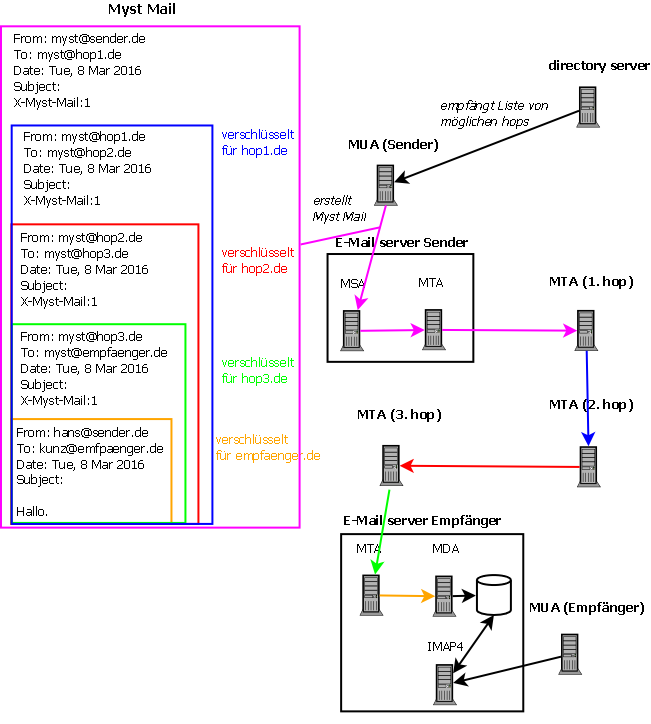
\includegraphics[scale=0.5]{Content/Entwicklung/IdeaConcept/Algorithmus.png}
	\caption{Übersicht MystMail Algorithmus}
	\label{fig:algorithmus}
\end{figure}
\vfill
\clearpage